\documentclass[a4paper,12pt]{article}
  \usepackage[margin=2cm]{geometry}
  \usepackage[parfill]{parskip}
  \usepackage[utf8]{inputenc}
  \usepackage[sorting=none]{biblatex}
    \addbibresource{protocol.bib}
  \usepackage{hyperref}
    \hypersetup{
      colorlinks=true,
      pdftitle={Protocol Berg},
    }
  \usepackage{hologo}
  \usepackage{graphicx}
  \usepackage{caption}
  \usepackage{subcaption}

  \title{\huge \textbf{Protocol Berg}\\[.5em]
    \large \textit{The decentralized protocol and infrastructure conference.\\
     Revision 0b11111100111.}}
  \author{Satoshi Nakamoto, Vitalik Buterin, Juan Benet, Molly Mackinley,\\
    Gavin Wood, Robert Habermeier, Ethan Buchanan, Zaki Manian, Jae Kwon,\\
    et alia.\\[1em]\textit{A Department of Decentralization \cite{dod} Event.}}
  \date{September 15, 2023, Kreuzberg, Berlin.}

\begin{document}
  \maketitle

  \begin{abstract}
    There are various conferences addressing end-user applications and consumer-grade products
    \cite{dapp}\cite{desci}\cite{bbw}.
    However, not many of them manage to create a stage for protocol research, decentralized
    infrastructure, or core-developer experience. Protocol Berg is a novel summit to address this
    shortcoming by creating a one-day event with two parallel stages and several opportunities for
    technical workshops and protocol community gatherings. Attendance is free of charge and the
    event will not be influenced by sponsors or commercial vendors.
  \end{abstract}

  \section{Conference}

\begin{figure}
  \centering
  \begin{subfigure}[t]{.3\linewidth}
    \centering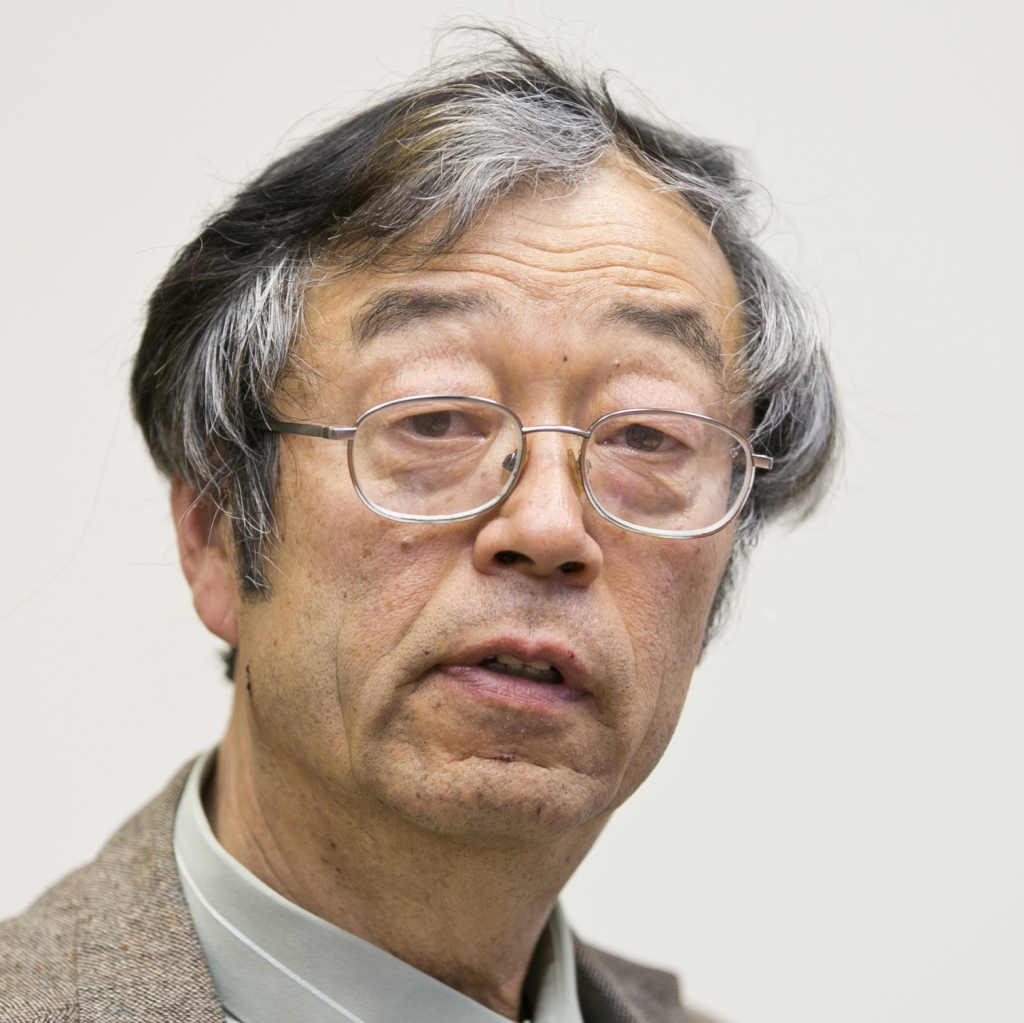
\includegraphics[width=.5\linewidth]{img/satoshi}
    \caption{\textbf{Satoshi Nakamoto}, Bitcoin, A Peer-to-Peer, Electronic Cash System.}
  \end{subfigure}
  \begin{subfigure}[t]{.3\linewidth}
    \centering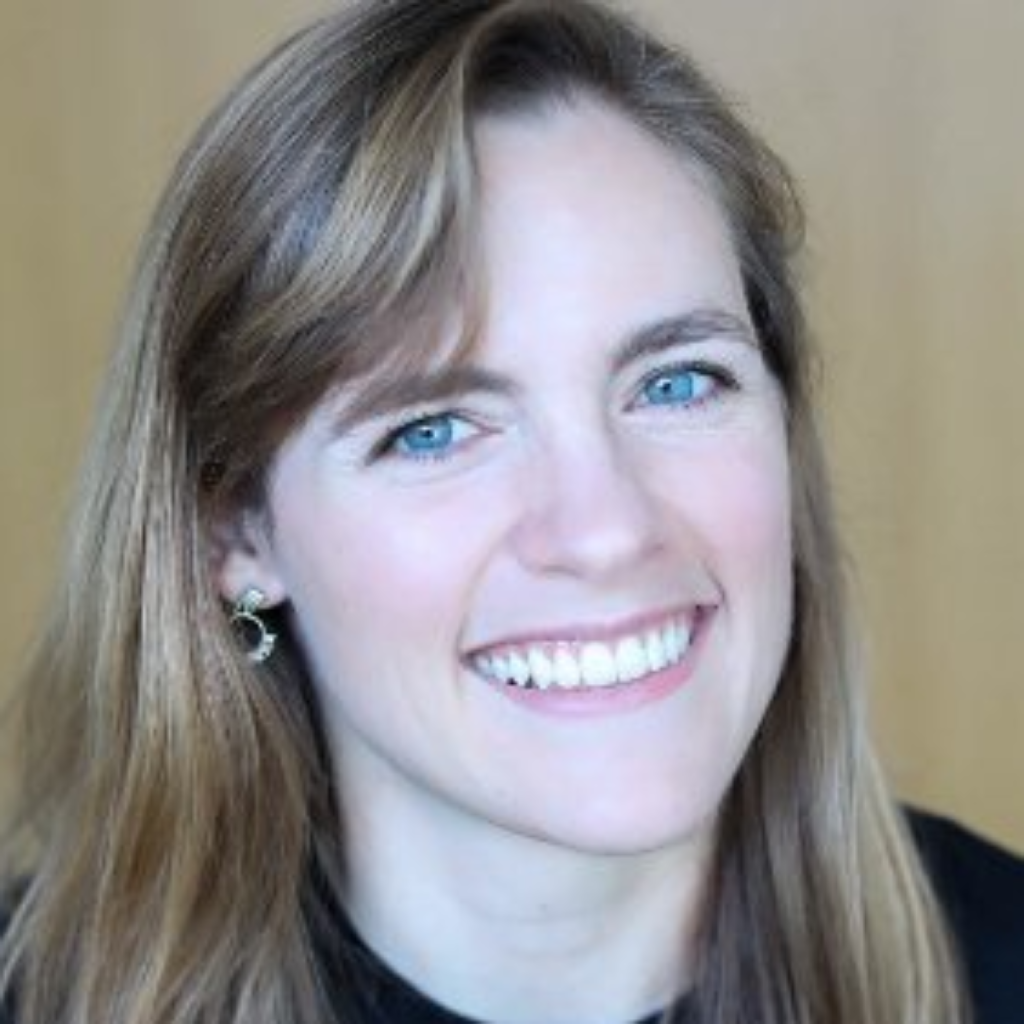
\includegraphics[width=.5\linewidth]{img/molly}
    \caption{\textbf{Molly Mackinlay}, IPFS, A Content-Addressed, Versioned, Peer-to-Peer File System.}
  \end{subfigure}
  \begin{subfigure}[t]{.3\linewidth}
    \centering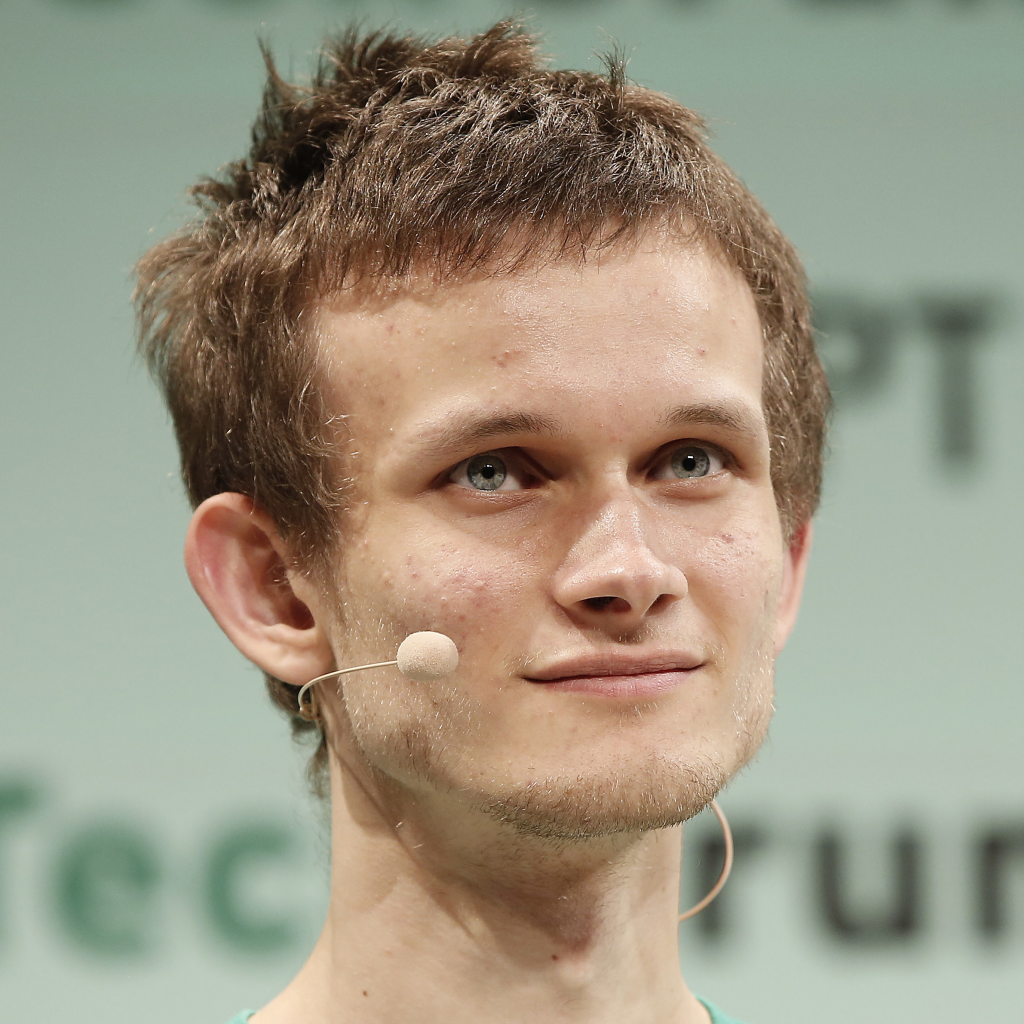
\includegraphics[width=.5\linewidth]{img/vitalik}
    \caption{\textbf{Vitalik Buterin}, Ethereum, A Next-Generation Smart Contract, Decentralized Application Platform.}
  \end{subfigure}

  \medskip

  \begin{subfigure}[t]{.3\linewidth}
    \centering
\includegraphics[width=.5\linewidth]{img/megan}
    \caption{\textbf{Megan Klimen}, Filecoin, A Decentralized Storage Network.}
  \end{subfigure}
  \begin{subfigure}[t]{.3\linewidth}
    \centering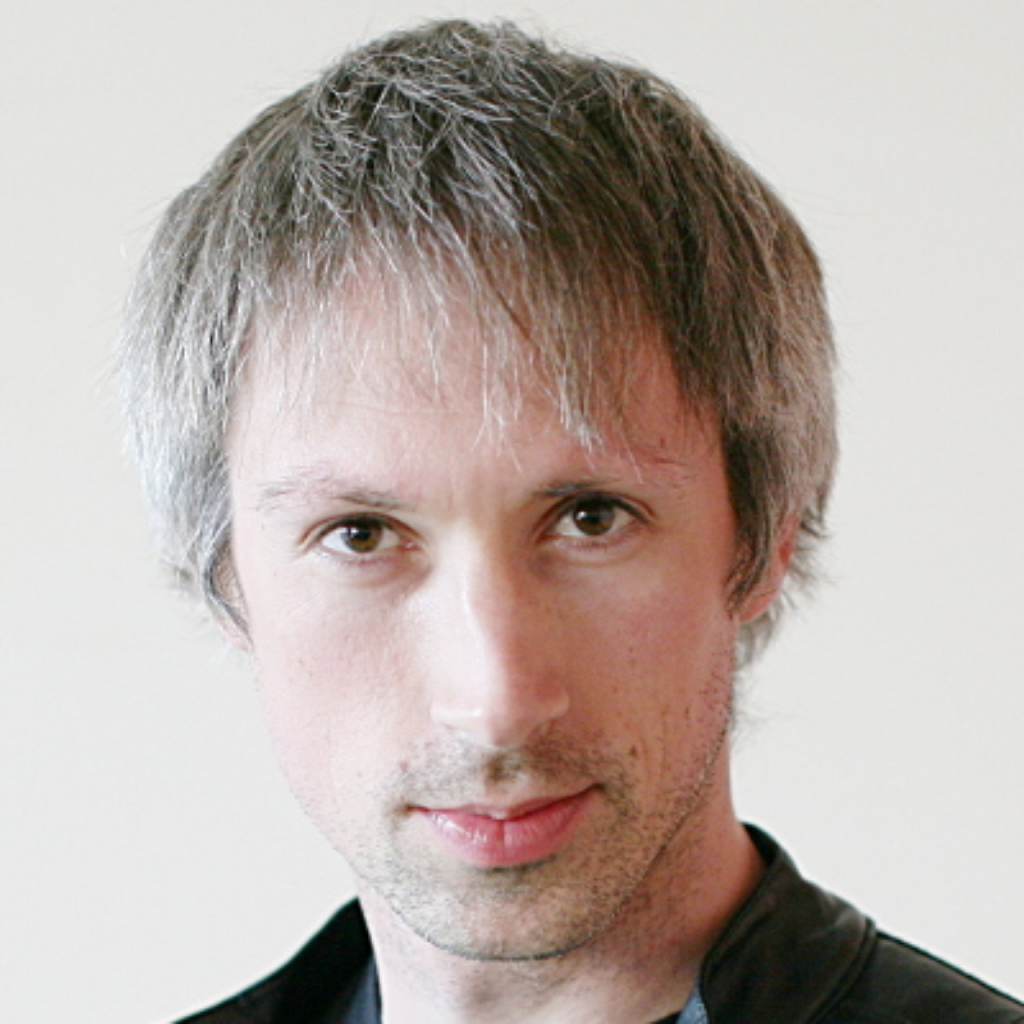
\includegraphics[width=.5\linewidth]{img/gavin}
    \caption{\textbf{Gavin Wood}, Polkadot, A Heterogeneous Multi-Chain Framework.}
  \end{subfigure}
  \begin{subfigure}[t]{.3\linewidth}
    \centering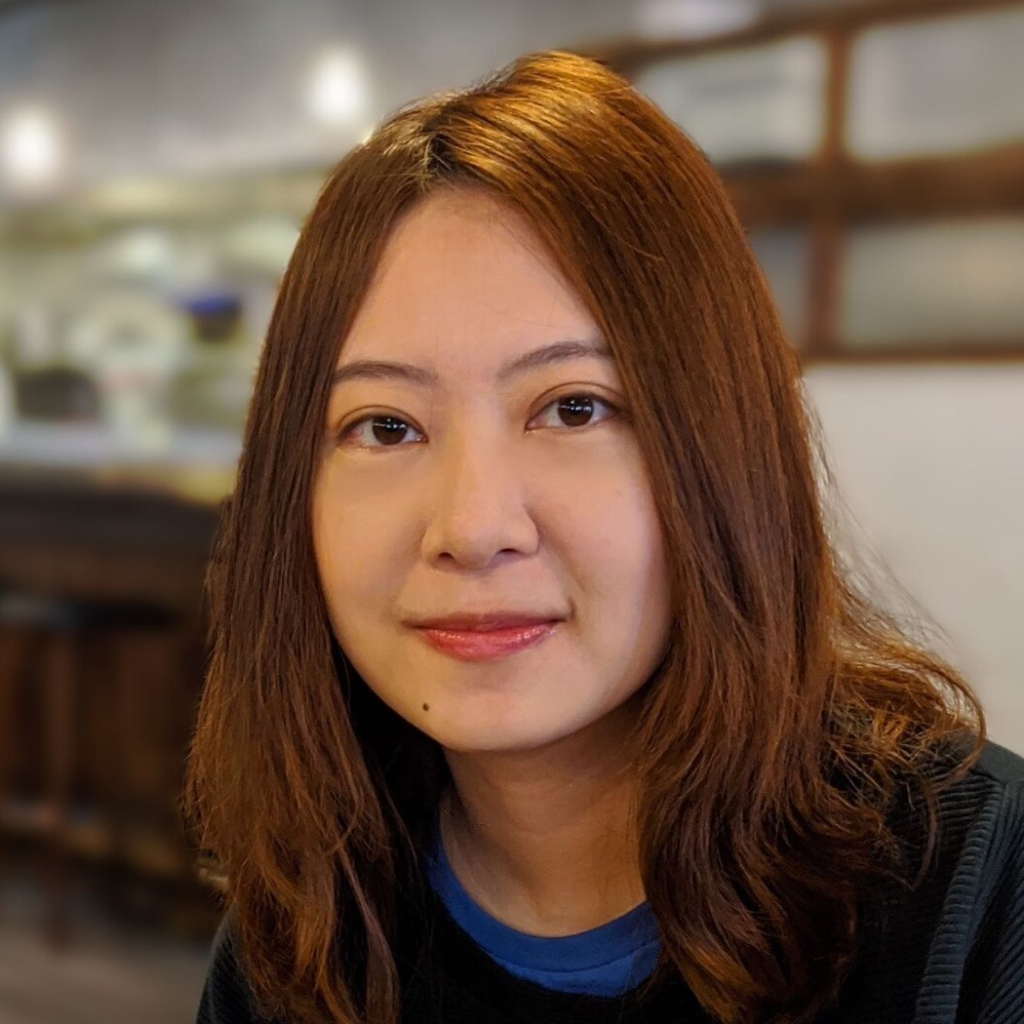
\includegraphics[width=.5\linewidth]{img/hsiao}
    \caption{\textbf{Hsiao-Wei Wang}, Ethereum, A Next-Generation Smart Contract, Decentralized Application Platform.}
  \end{subfigure}

  \caption{Speakers of Protocol Berg, 2023.}
  \end{figure}

  Protocol Berg will be a one-day technical conference targeting an audience of protocol engineers,
  system engineers, network engineers, blockchain operation engineers, decentralized
  infrastructure administrators, as well as researchers and other curious minds.

  Topics covered by the event orbit mainly around consensus protocols, distributed virtual
  machines, peer-to-peer networking, decentralized infrastructure, open-source governance, and
  protocol research.

  The venue will be equipped with two stages, one for keynotes, visionary talks, and events, and
  one for hands-down technical talks. In addition, there will be workshop areas for deep technical
  study and knowledge-sharing classes.

  We expect 500-600 attendees and tickets will be free as in \textit{free lemonade}. There will
  be no sponsors and no swag, or any other distractions whatsoever.

  \section{Call for Participation}
  To submit a technical talk or workshop proposal, use our Pretalx interface:\\
  \hspace*{3em}\url{https://speak.protocol.berlin}

  To join our collective as contributor or volunteer, please email us:\\
  \hspace*{3em}\url{hello@ethberlin.org}

  \section{Venue}
  The \textit{Heeresbäckerei} (magazine in the army bakery) \cite{backen} in Berlin-Kreuzberg is
  an impressive industrial monument located directly at the Spree. The magazine in the west wing
  was used as a warehouse since 1890, lorries with flour and grain traveled on rails between the
  magazine and the bakery. The brick building has retained its substance over the years. Cast iron
  columns carry a five-meter-high ceiling, the parquet is made of old beech, deep arched windows
  open the room to the light.

  The result is a magnificent hall with a good deal of charm – perhaps the most beautiful in
  Berlin-Kreuzberg \cite{xberg}. \textbf{Address: Köpenicker Straße 16-17, 10997 Berlin-Kreuzberg}.

  \section{About the Host}
  The \textit{Department of Decentralization} \cite{dod} is a collective of people from various
  crypto, decentralization, and blockchain communities in and around Berlin. The group first
  assembled in 2018 to organize events such as ETHBerlin \cite{ethberlin} or GoerliCon
  \cite{goerli} and has been active since.

  The aim is to be an agnostic vehicle to drive adoption, educate newcomers, and raise awareness
  on the challenges and benefits of decentralization and open source software. Currently, the
  Department is primarily run from Berlin. The collective is composed of around a dozen members
  and takes decisions using rough consensus.

  \section{Impressum}
  Angaben gemäß § 5 TMG: Goerli Dezentral gGmbH, Mariannenstraße 9-10, 10999 Berlin,
  Handelsregister: HRB 207663 B, Registergericht: Amtsgericht Charlottenburg, Berlin,
  Umstatzsteuer-ID: DE325917754, vertreten durch Afri Schoedon, \url{schoedon@ethberlin.org},
  +49 (0)30 20613410.

  Goerli Dezentral gGmbH is a non-profit organization serving tax-privileged
  purposes, according to the articles of association. The organization meets the statutory
  requirements under §§ 51, 59, 60, and 61 AO in Germany.

  \section{Foo Bar Baz}
  \LaTeX's default font is Computer Modern \cite{font}, but the editor also supports a
  number of other font types.

  \printbibliography
\end{document}
